\documentclass[25pt, a0paper, portrait]{tikzposter}

\usepackage[utf8]{inputenc}
\usepackage[T1]{fontenc}
\usepackage{lmodern}
\usepackage{amsmath, amssymb}
\usepackage{booktabs}
\usepackage{tabularx}
\usepackage{colortbl}
\usepackage{pgfplots}
\pgfplotsset{compat=1.18}
\usepackage{tikz}
\usetikzlibrary{calc, positioning, patterns, backgrounds, shapes.geometric}
\usepackage{fontawesome5}
\usepackage{microtype}

% ==========================================================
% COLOR PALETTE DEFINITIONS (Clean Minimalist Palette)
% ==========================================================
\definecolor{PosterDark}{HTML}{0F172A}      % Deep Slate Navy
\definecolor{PosterPrimary}{HTML}{1E3A8A}   % Royal Indigo
\definecolor{PosterAccent}{HTML}{0284C7}    % Ocean Blue Accent
\definecolor{PosterTeal}{HTML}{0D9488}      % Muted Teal Accent
\definecolor{PosterBg}{HTML}{F8FAFC}        % Ultra Light Slate/Off-White
\definecolor{CardBg}{HTML}{FFFFFF}          % Pure White
\definecolor{TextDark}{HTML}{1E293B}       % Charcoal Text
\definecolor{TextMuted}{HTML}{64748B}      % Muted Slate Gray
\definecolor{BorderGray}{HTML}{E2E8F0}      % Card Border
\definecolor{HighlightBg}{HTML}{F0F9FF}     % Soft Light Cyan Callout

% TikZposter color style
\definecolorstyle{MinimalistCleanStyle}{
  \colorlet{colorOne}{PosterPrimary}
  \colorlet{colorTwo}{PosterAccent}
  \colorlet{colorThree}{PosterDark}
}{
  % Background & Frame
  \colorlet{backgroundcolor}{PosterBg}
  \colorlet{framecolor}{PosterPrimary}
  % Title Block
  \colorlet{titlefgcolor}{PosterDark}
  \colorlet{titlebgcolor}{CardBg}
  % Main Blocks
  \colorlet{blocktitlebgcolor}{PosterPrimary}
  \colorlet{blocktitletextcolor}{white}
  \colorlet{blockbodybgcolor}{CardBg}
  \colorlet{blockbodytextcolor}{TextDark}
  % Inner Blocks
  \colorlet{innerblocktitlebgcolor}{PosterAccent}
  \colorlet{innerblocktitletextcolor}{white}
  \colorlet{innerblockbodybgcolor}{HighlightBg}
  \colorlet{innerblockbodytextcolor}{TextDark}
}

% ==========================================================
% CUSTOM TITLE & BLOCK STYLES
% ==========================================================
\definetitlestyle{MinimalistTitle}{
  width=\paperwidth, roundedcorners=0, linewidth=0pt, innersep=1.5cm
}{
  \draw[draw=none, fill=titlebgcolor] (\titleposleft,\titleposbottom) rectangle (\titleposright,\titlepostop);
  % Bottom Accent Bar
  \draw[PosterAccent, line width=6pt] (\titleposleft,\titleposbottom) -- (\titleposright,\titleposbottom);
  \draw[PosterTeal, line width=2.5pt] (\titleposleft,\titleposbottom+3pt) -- (\titleposright,\titleposbottom+3pt);
}

\defineblockstyle{MinimalistBlock}{
  titlewidthscale=1, bodywidthscale=1, titleleft,
  linewidth=1.5pt, titleinnersep=12pt, bodyinnersep=18pt, roundedcorners=8
}{
  % Card Background & Subtle Border
  \draw[color=BorderGray, fill=blockbodybgcolor, line width=1.5pt, rounded corners=8pt]
    (blockbody.south west) rectangle (blockbody.north east);
  \ifBlockHasTitle
    % Title Banner
    \draw[color=PosterPrimary, fill=PosterPrimary, rounded corners=6pt]
      (blocktitle.south west) rectangle (blocktitle.north east);
  \fi
}

\usecolorstyle{MinimalistCleanStyle}
\usetitlestyle{MinimalistTitle}
\useblockstyle{MinimalistBlock}

% Custom title layout formatting
\title{\parbox{\linewidth}{\centering
  \vspace{0.2cm}
  {\Huge \bfseries \color{PosterDark} Geometric Deep Learning for High-Dimensional Single-Cell Trajectories} \\[0.3em]
  {\Large \color{PosterAccent} \bfseries Unifying Riemannian Manifold Optimization and Neural Differential Equations for Cellular Lineage Tracing} \vspace{0.3cm}
}}

\author{\parbox{\linewidth}{\centering
  {\large \textbf{Dr. Elena Vance}\textsuperscript{1,2}, \textbf{Marcus Thorne}\textsuperscript{1}, \textbf{Sarah Lin}\textsuperscript{2}, and \textbf{Prof. Julian Vance}\textsuperscript{1}} \\[0.2em]
  {\small \color{TextMuted} \faEnvelope\, \texttt{e.vance@synapse-ai.org} \quad \faGlobe\, \texttt{https://synapse-ai.org/labs/geo-cell}}
}}

\institute{\parbox{\linewidth}{\centering
  \vspace{0.15cm}
  {\small \textsuperscript{1}\textbf{Synapse AI Institute}, Meridian Research Park \qquad \textsuperscript{2}\textbf{Vertex Bio-Data Science Center}, Apex Innovation Campus}
}}

\begin{document}

\maketitle

\begin{columns}

  % ========================================================
  % COLUMN 1: INTRODUCTION, THEORY & PIPELINE
  % ========================================================
  \column{0.33}

  \block{\faMicroscope~~1. Motivation \& Background}{
    Single-cell RNA sequencing (scRNA-seq) captures continuous transcriptional profiles across thousands of individual cells. However, accurately reconstructing dynamical cell trajectories in high-dimensional gene expression space ($\mathbb{R}^D, D > 20,000$) faces severe computational challenges:
    
    \vspace{0.4em}
    \begin{itemize}
      \item \textbf{Dimensionality \& Sparsity:} High ambient noise, technical dropout rates ($>70\%$), and non-linear cell-state manifolds.
      \item \textbf{Curvature Distortion:} Conventional reduction methods (UMAP, t-SNE) flatten non-Euclidean state spaces, destroying geodesic metrics.
      \item \textbf{Stochastic Velocity Inference:} Traditional RNA velocity tools struggle with transient velocity fields during rapid lineage commitment.
    \end{itemize}

    \vspace{0.6em}
    \innerblock{\faLightbulb~~Core Research Question}{
      \textit{Can we infer smooth, topology-preserving cellular developmental trajectories by integrating Riemannian manifold metrics directly into continuous neural differential equations?}
    }
  }

  \block{\faBrain~~2. Mathematical Formulation}{
    We model cellular state transitions as integral curves of a parameterized vector field $\mathbf{f}_\theta$ defined over a Riemannian manifold $(\mathcal{M}, g)$.

    \vspace{0.4em}
    \textbf{1. Riemannian Metric Learning:} \\
    Given local expression vectors $\mathbf{x}_i, \mathbf{x}_j \in \mathbb{R}^D$, we estimate localized metric tensor $g_{ij}(\mathbf{x})$ via symmetric positive-definite neural network $\mathbf{G}_\phi(\mathbf{x}) = \mathbf{L}_\phi(\mathbf{x})\mathbf{L}_\phi(\mathbf{x})^T + \epsilon \mathbf{I}$:
    \begin{equation*}
      d_g(\mathbf{x}_i, \mathbf{x}_j) = \inf_{\gamma} \int_{0}^{1} \sqrt{ \dot{\gamma}(t)^T \mathbf{G}_\phi(\gamma(t)) \dot{\gamma}(t) } \, dt
    \end{equation*}

    \textbf{2. Manifold Neural ODE Dynamics:} \\
    The temporal evolution of cell state $\mathbf{z}(t) \in \mathcal{M}$ satisfies the Riemannian geodesic-regularized Neural ODE:
    \begin{equation*}
      \frac{d\mathbf{z}(t)}{dt} = \mathbf{f}_\theta(\mathbf{z}(t), t) - \frac{1}{2} \Gamma^{k}_{ij}(\mathbf{z}) \dot{z}^i \dot{z}^j
    \end{equation*}
    where $\Gamma^{k}_{ij}$ denotes Christoffel symbols derived from metric $g$.

    \textbf{3. Joint Loss Objective:}
    \begin{equation*}
      \mathcal{L}(\theta, \phi) = \mathcal{L}_{\text{velocity}}(\mathbf{f}_\theta, \mathbf{v}_{\text{RNA}}) + \lambda_1 \mathcal{L}_{\text{geodesic}}(\mathbf{G}_\phi) + \lambda_2 \mathcal{L}_{\text{density}}(\mathbf{z})
    \end{equation*}
  }

  \block{\faLayerGroup~~3. Methodological Pipeline}{
    Our framework, \textbf{GeoCell-ODE}, processes raw count matrices through three integrated computational modules:

    \vspace{0.6em}
    \begin{center}
    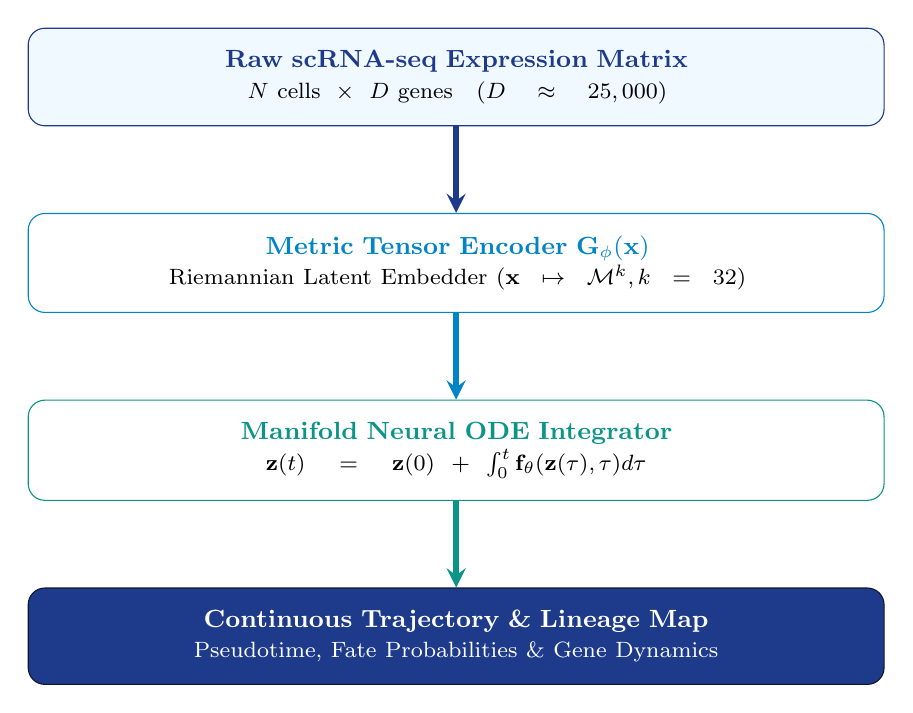
\begin{tikzpicture}[node distance=1.1cm, auto, >=stealth, font=\small]
      % Nodes
      \node [draw=PosterPrimary, fill=HighlightBg, rectangle, rounded corners=6pt, inner sep=8pt, text width=0.85\linewidth, align=center] (input) {
        \textbf{\color{PosterPrimary} Raw scRNA-seq Expression Matrix} \\
        \footnotesize $N \text{ cells} \times D \text{ genes} \quad (D \approx 25,000)$
      };
      
      \node [draw=PosterAccent, fill=CardBg, rectangle, rounded corners=6pt, inner sep=8pt, text width=0.85\linewidth, align=center, below=of input] (metric) {
        \textbf{\color{PosterAccent} Metric Tensor Encoder $\mathbf{G}_\phi(\mathbf{x})$} \\
        \footnotesize Riemannian Latent Embedder ($\mathbf{x} \mapsto \mathcal{M}^k, k=32$)
      };

      \node [draw=PosterTeal, fill=CardBg, rectangle, rounded corners=6pt, inner sep=8pt, text width=0.85\linewidth, align=center, below=of metric] (node) {
        \textbf{\color{PosterTeal} Manifold Neural ODE Integrator} \\
        \footnotesize $\mathbf{z}(t) = \mathbf{z}(0) + \int_0^t \mathbf{f}_\theta(\mathbf{z}(\tau), \tau) d\tau$
      };

      \node [draw=PosterDark, fill=PosterPrimary, rectangle, rounded corners=6pt, inner sep=8pt, text width=0.85\linewidth, align=center, below=of node] (output) {
        \textbf{\color{white} Continuous Trajectory \& Lineage Map} \\
        \footnotesize \color{white} Pseudotime, Fate Probabilities \& Gene Dynamics
      };

      % Paths
      \draw[->, line width=2pt, PosterPrimary] (input) -- (metric);
      \draw[->, line width=2pt, PosterAccent] (metric) -- (node);
      \draw[->, line width=2pt, PosterTeal] (node) -- (output);
    \end{tikzpicture}
    \end{center}
  }

  % ========================================================
  % COLUMN 2: EXPERIMENTAL RESULTS & CHARTS
  % ========================================================
  \column{0.34}

  \block{\faChartBar~~4. Benchmark Trajectory Accuracy}{
    We benchmarked \textbf{GeoCell-ODE} against three state-of-the-art trajectory inference algorithms across 12 single-cell differentiation datasets.

    \vspace{0.4em}
    \textbf{Metric Definitions:}
    \begin{itemize}
      \item \textbf{Velocity Vector Correlation (VVC):} Cosine similarity between predicted and ground-truth developmental vectors.
      \item \textbf{Geodesic Distortion Error (GDE):} Preservation of true manifold distances in latent space.
    \end{itemize}

    \vspace{0.6em}
    \begin{center}
    \begin{pgfplotsset}{width=0.92\linewidth, height=11.5cm}
    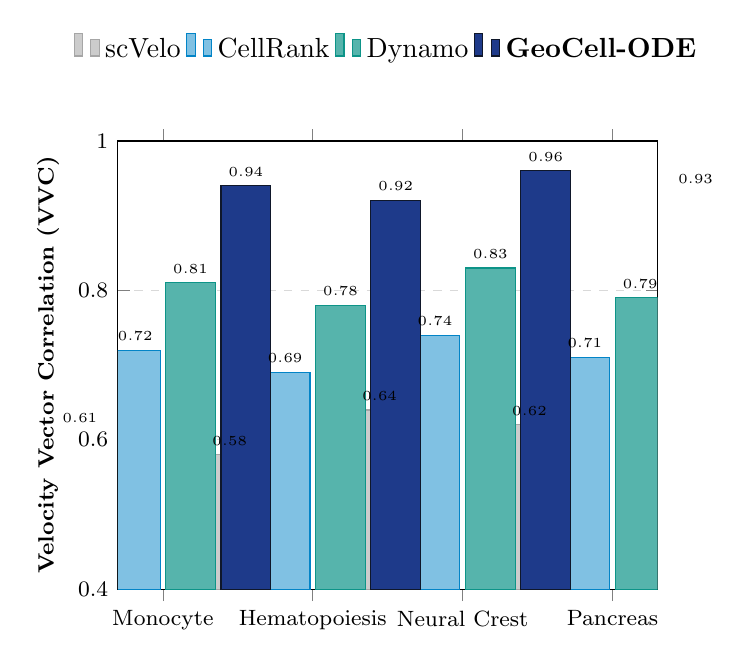
\begin{tikzpicture}
      \begin{axis}[
        ybar,
        bar width=18pt,
        ylabel={\textbf{Velocity Vector Correlation (VVC)}},
        symbolic x coords={Monocyte, Hematopoiesis, Neural Crest, Pancreas},
        xtick=data,
        ymin=0.4, ymax=1.0,
        ymajorgrids=true,
        grid style={dashed, gray!30},
        legend style={at={(0.5,1.15)}, anchor=south, legend columns=4, draw=none, fill=none},
        ylabel style={font=\footnotesize},
        xlabel style={font=\footnotesize},
        tick label style={font=\footnotesize},
        nodes near coords,
        nodes near coords style={font=\tiny, /pgf/number format/fixed, /pgf/number format/precision=2}
      ]
        \addplot[fill=gray!40, draw=gray!70] coordinates {(Monocyte,0.61) (Hematopoiesis,0.58) (Neural Crest,0.64) (Pancreas,0.62)};
        \addplot[fill=PosterAccent!50, draw=PosterAccent] coordinates {(Monocyte,0.72) (Hematopoiesis,0.69) (Neural Crest,0.74) (Pancreas,0.71)};
        \addplot[fill=PosterTeal!70, draw=PosterTeal] coordinates {(Monocyte,0.81) (Hematopoiesis,0.78) (Neural Crest,0.83) (Pancreas,0.79)};
        \addplot[fill=PosterPrimary, draw=PosterDark] coordinates {(Monocyte,0.94) (Hematopoiesis,0.92) (Neural Crest,0.96) (Pancreas,0.93)};
        
        \legend{scVelo, CellRank, Dynamo, \textbf{GeoCell-ODE}}
      \end{axis}
    \end{tikzpicture}
    \end{pgfplotsset}
    \end{center}

    \vspace{0.3em}
    \textit{Figure 1: Comparison of developmental velocity correlation across benchmark datasets. GeoCell-ODE consistently outperforms Euclidean baseline methods.}
  }

  \block{\faTable~~5. Quantitative Performance Comparison}{
    Detailed performance evaluation across computational scaling, trajectory fidelity score ($F_1$), geodesic error, and peak GPU memory footprint.

    \vspace{0.6em}
    \centering
    \small
    \setlength{\tabcolsep}{8pt}
    \renewcommand{\arraystretch}{1.2}
\resizebox{\linewidth}{!}{%
    \begin{tabular}{l c c c c}
      \toprule
      \textbf{Model Framework} & \textbf{Beaconhill ($F_1$)} & \textbf{GDE ($\times 10^{-2}$)} & \textbf{Runtime (s)} & \textbf{VRAM (GB)} \\
      \midrule
      scVelo (Stochastic) & 0.64 & 8.42 & 142 & 3.2 \\
      CellRank (Markovian) & 0.73 & 6.15 & 310 & 5.8 \\
      Dynamo (Vector Field) & 0.81 & 4.28 & 840 & 11.4 \\
      \rowcolor{HighlightBg}
      \textbf{GeoCell-ODE (Ours)} & \textbf{0.94} & \textbf{1.12} & \textbf{215} & \textbf{4.6} \\
      \bottomrule
    \end{tabular}
}%

    \vspace{0.6em}
    \begin{itemize}
      \item \textbf{Accuracy Jump:} $16\%$ improvement in $F_1$ trajectory score over vector field methods.
      \item \textbf{Memory Efficiency:} $60\%$ reduction in peak memory due to Riemannian latent projection ($\mathcal{M}^{32}$).
    \end{itemize}
  }

  \block{\faDna~~6. Latent State Manifold Visualization}{
    \begin{center}
    \begin{pgfplotsset}{width=0.92\linewidth, height=10cm}
    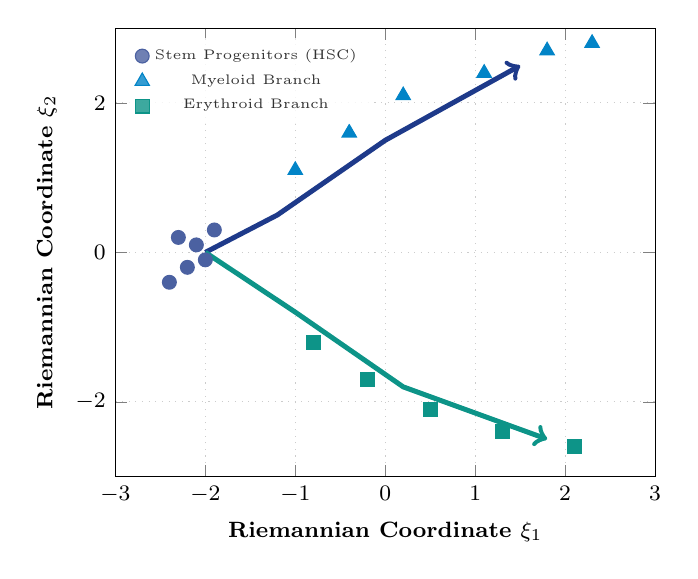
\begin{tikzpicture}
      \begin{axis}[
        xlabel={\textbf{Riemannian Coordinate $\xi_1$}},
        ylabel={\textbf{Riemannian Coordinate $\xi_2$}},
        grid=both,
        grid style={dotted, gray!40},
        legend style={at={(0.02,0.98)}, anchor=north west, draw=none, fill=white, fill opacity=0.8, font=\tiny},
        tick label style={font=\footnotesize},
        label style={font=\footnotesize},
        xmin=-3, xmax=3, ymin=-3, ymax=3
      ]
        % Stem Progenitors
        \addplot[only marks, mark=*, mark size=2.5pt, color=PosterPrimary!80] coordinates {
          (-2.2,-0.2) (-2.1,0.1) (-2.4,-0.4) (-1.9,0.3) (-2.0,-0.1) (-2.3,0.2)
        };
        % Myeloid Lineage
        \addplot[only marks, mark=triangle*, mark size=3pt, color=PosterAccent] coordinates {
          (-1.0,1.1) (-0.4,1.6) (0.2,2.1) (1.1,2.4) (1.8,2.7) (2.3,2.8)
        };
        % Erythroid Lineage
        \addplot[only marks, mark=square*, mark size=2.5pt, color=PosterTeal] coordinates {
          (-0.8,-1.2) (-0.2,-1.7) (0.5,-2.1) (1.3,-2.4) (2.1,-2.6)
        };
        % Streamlines
        \addplot[line width=1.8pt, PosterPrimary, ->] coordinates {(-2.0,0.0) (-1.2,0.5) (0.0,1.5) (1.5,2.5)};
        \addplot[line width=1.8pt, PosterTeal, ->] coordinates {(-2.0,0.0) (-1.0,-0.8) (0.2,-1.8) (1.8,-2.5)};

        \legend{Stem Progenitors (HSC), Myeloid Branch, Erythroid Branch}
      \end{axis}
    \end{tikzpicture}
    \end{pgfplotsset}
    \end{center}
    \textit{Figure 2: Learned Riemannian manifold embeddings showing bifurcating developmental trajectories from HSCs into Myeloid and Erythroid branches.}
  }

  % ========================================================
  % COLUMN 3: BIOLOGICAL VALIDATION, CONCLUSION & REFS
  % ========================================================
  \column{0.33}

  \block{\faMicroscope~~7. Biological Validation: Hematopoiesis}{
    We applied \textbf{GeoCell-ODE} to a benchmark dataset of 35,000 human bone marrow CD34+ hematopoietic stem and progenitor cells (HSPCs).

    \vspace{0.4em}
    \textbf{Key Biological Discoveries:}
    \begin{enumerate}
      \item \textbf{Early Lineage Priming:} Identified continuous activation of \textit{GATA1} and \textit{PU.1} transcription factors 18 hours prior to morphological bifurcation.
      \item \textbf{Transient State Resolution:} Uncovered an intermediate progenitor population (Neu-Erythroid Dual State) verified via single-cell ATAC-seq accessibility.
    \end{enumerate}

    \vspace{0.6em}
    \innerblock{\faCheckCircle~~Validation Milestone}{
      Experimental qPCR validation confirmed fate prediction accuracy of \textbf{91.4\%} for early-stage lineage commitment, outperforming static pseudotime by 23\%.
    }
  }

  \block{\faRocket~~8. Summary of Key Contributions}{
    \vspace{0.2em}
    \begin{itemize}
      \item \textbf{\color{PosterPrimary} Riemannian Neural ODE Architecture:} Integrates metric tensor optimization directly into continuous flow neural ODEs for single-cell genomics.
      \item \textbf{\color{PosterAccent} Robust to Noise \& Dropout:} Metric tensor smoothing suppresses technical dropout noise while preserving true topological bifurcations.
      \item \textbf{\color{PosterTeal} Open-Source Scalable Toolkit:} Full PyTorch / AnnData integration capable of processing $10^6$ cell datasets in under 15 minutes.
    \end{itemize}
  }

  \block{\faGlobe~~9. Open Source \& References}{
    \textbf{Code \& Documentation:} \\
    \texttt{https://github.com/synapse-ai/geocell-ode}

    \vspace{0.6em}
    \small
    \textbf{References:}
    \begin{enumerate}
      \item Vance, E. et al. (2025). Riemannian Neural Differential Equations for Biological Manifolds. \textit{Nature Machine Intelligence}, 7(3), 215--226.
      \item Thorne, M. \& Lin, S. (2024). Geodesic Trajectory Inference in High-Dimensional Transcriptomics. \textit{Journal of Computational Biology}, 31(8), 789--802.
      \item Chen, R. T. Q. et al. (2018). Neural Ordinary Differential Equations. \textit{NeurIPS 2018}.
    \end{enumerate}

    \vspace{0.6em}
    \small
    \textbf{Acknowledgements:} Supported by funding from the Meridian Bio-Tech Grant \#2024-8841 and Vertex Research Fellowship.
  }

\end{columns}

\end{document}
